\documentclass[12pt]{article}

\usepackage{mystyle}
\usepackage{fancyvrb}
\usepackage{tikz}
\hypersetup{
    colorlinks=true,
    urlcolor=blue,
    }

\renewcommand{\algorithmicrequire}{\textbf{Inputs:}}
%\renewcommand{\algorithmiccomment}[1]{// #1}
\VerbatimFootnotes

\title{Optimizing Computing the $Q$ Factor in LAPACK}
\author{Johnathan Rhyne\\ Advised by: Julien Langou}


% Add talking about org2r against orgqr 


\begin{document}
    \maketitle
    \begin{abstract}
    Computing the Q factor from a sequence of Householder elementary reflections is an important operation for some 
    applications. We present new algorithms which speed up the performance of these operations. In addition, we also 
    implement existing algorithms originally developed by Puglisi to speed up the computation of the T matrix. We see 
    performance improvements on the order of 2 to 5 times more efficiency in comparison to the reference LAPACK 
    computations and see similar performance in many cases as the optimized implementation for AMD (AOCL). Using these 
    schemes we not only see an improvement in execution time, but lowers the memory footprint for the main driver 
    algorithm.
    \end{abstract}
    \section{Preliminaries}
    We use householder reflectors to represent orthogonal matrices as a product of $k$ many rank one updates to the identity matrix. This means we can write an orthogonal matrix $Q_m\in\R^{m\times m}$ as 
    \begin{equation}\label{eq:Q}
        Q_m = \left(I - \tau_1 v_1v_1^\top\right)\cdots\left(I - \tau_kv_kv_k^\top\right)
    \end{equation}
    One key note is that if we don't want all $m$ of the columns, we can instead choose a smaller amount denoted $n$ 
    and this lets us get $Q_n\in\R^{m\times n}$ by 
    \begin{equation}\label{eq:Qn}
        Q_n = \left(I - \tau_1 v_1v_1^\top\right)\cdots\left(I - \tau_kv_kv_k^\top\right)I_{m\times n}
    \end{equation}
    Where the $i,j$th element of $I_{m\times n}$ is given by:
    \begin{equation*}
        I_{m\times n}(i,j) = \begin{cases}
            1 & 1\leq i = j\leq n\\
            0 & \text{otherwise}
        \end{cases}
    \end{equation*}
    Throughout this discussion, we will omit the subscripts, and instead we will be assuming the size to be 
    what makes sense in context. In general, algorithms will compute $Q_n$ while our theory will discuss computing $Q_m$. 
    and we will assume that $m\geq n\geq k$.
    \section{DORGQR Overview}
    \subsection{Motivation}
    At a high level, we want to compute this matrix. One method is to compute $Q$ is given by algorithm \ref{alg:dorg2r}

    \begin{algorithm}
        \caption{Columnwise computation of $Q$}\label{alg:dorg2r}
        \begin{algorithmic}[1]
            \STATE $Q= I_{m\times n}$
            \FOR{$i=k,\dots,1$}
                \STATE $Q= \left(I-\tau_iv_iv_i^\top\right)Q$
            \ENDFOR
        \end{algorithmic}
    \end{algorithm}

    A proper implementation of algorithm \ref{alg:dorg2r} will do so via matrix-vector products. While these operations
    are heavily optimized, we can still gain more by instead trying to use matrix-matrix
    operations. So, we look at how we can combine a few loops from algorithm \ref{alg:dorg2r}. In order to motivate the general method we first look at the case of $k=2$.

    When this happens, we see that equation \ref{eq:Q} gives us the following
    \begin{align*}
        Q &= \left(I-\tau_1v_1v_1^\top\right)\left(I-\tau_2v_2v_2^\top\right) \\
        &= I - \tau_1v_1v_1^\top - \tau_2v_2v_2^\top + \tau_1\tau_2v_1v_1^\top v_2v_2^\top
    \end{align*}
    Defining the matrices
    \begin{align*}
        V &= \begin{bmatrix} v_1 & v_2 \end{bmatrix} \\
        T &= \begin{bmatrix}
            \tau_1 & \tau_1\tau_2v_1^\top v_2 \\
            0      & \tau_2
        \end{bmatrix}
    \end{align*}
    We can rewrite above as 
    \[
        Q = I - VTV^\top
    \]
    In fact, we can extend this even further to the case where we assume we already collected some of our reflectors and we now want to collect these ``blocks''
    \begin{align*}
        Q &= \left(I - V_1T_{1,1}V_1^\top\right)\left(I - V_2T_{2,2}V_2^\top\right) \\
        &= I - V_1T_{1,1}V_1^\top - V_2T_{2,2}V_2^\top + V_1T_{1,1}V_1^\top V_2T_{2,2}V_2^\top \\
        &= I - V_1T_{1,1}V_1^\top - V_2T_{2,2}V_2^\top + V_1\left(T_{1,1}V_1^\top V_2T_{2,2}\right)V_2^\top 
    \end{align*}
    Similarly as above, we define the following matrices

    \begin{align*}
        V &= \begin{bmatrix} V_1 V_2 \end{bmatrix}\\
        T &= \begin{bmatrix} 
            T_{1,1} & T_{1,2} \\
            0       & T_{2,2}
        \end{bmatrix}
    \end{align*}
    Where 
    $$
    T_{1,2} = T_{1,1}V_1^\top V_2T_{2,2}.
    $$
    We see that 
    \[
        Q = I - VTV^\top
    \]
    \subsection{Existing Behavior}
    The way that $Q$ is computed in LAPACK is via algorithm \ref{alg:dorgqr}

    \begin{algorithm}
        \caption{Blocked computation of $Q$}\label{alg:dorgqr}
        \begin{algorithmic}[1]
            \STATE Determine blocking parameter $nb$
            \STATE $Q = I_{m\times n}$
            \FOR{Each block of size $nb$ of $V$ moving right to left}
                \STATE (\verb|DLARFT|) Compute $T$
                \STATE (\verb|DLARFB|) Apply $I-V_{nb}TV_{nb}^\top$ to the trailing columns of $Q$
                \STATE (\verb|DORG2R|) Apply $I-V_{nb}TV_{nb}^\top$ to itself
            \ENDFOR
        \end{algorithmic}
    \end{algorithm}

    Note: $V_{nb}$ is the current collection of $nb$ reflectors.

    The choice of $nb$ is an open question as to what is considered a ``good'' choice, in practice, $32$ is 
    the standard\footnote{To determine your own machine's blocksize for a given routine, see the interface for 
    \verb+ilaenv+ and call this function}. We don't investigate this choice much in this report, but we offer 
    some pointers to how investigating this choice could be beneficial.
    \subsection{Places for Optimization}
    Looking at algorithm \ref{alg:dorgqr}, we see $4$ main options for efficiency improvements. 
    \begin{enumerate}
        \item Improving the algorithm used inside \verb|DLARFT|
        \item Creating a specialized version of \verb|DLARBF|
        \item Rewriting the first iteration to exploit the fact that $Q$ was initialized as the identity.
        \item Replacing the call to \verb|DORG2R| with a call to a specialized block application to exploit $T$
    \end{enumerate}
    \section{Computation of T}
    Before we discuss the improvement of \verb|DLARFT|, we first motivate the current behavior which we will
    extend.
    
    Looking back at equation $\ref{eq:Q}$, we first consider the case of $k=2$, and see:
    \begin{align*}
        Q_m &= \left(I - \tau_1v_1v_1^\top\right)\left(I - \tau_2v_2v_2^\top\right) \\
            &= I - \tau_1v_1v_1^\top - \tau_2v_2v_2^\top + \tau_1v_1v_1^\top\tau_2v_2v_2^\top \\
            &= I - \tau_1v_1v_1^\top - \tau_2v_2v_2^\top + \left(\tau_1\tau_2v_1^\top v_2\right)v_1v_2^\top
    \end{align*}
    If we now define the matrices
    \begin{align*}
        V &= \begin{bmatrix} v_1 & v_2 \end{bmatrix} \\
            T &= \begin{bmatrix} \tau_1 & \tau_1\tau_2v_1^\top v_2 \\
            0 & \tau_2\end{bmatrix}.
    \end{align*}
    Then, we can rewrite equation \ref{eq:Q} as 
    \begin{equation}\label{eq:blockedQ}
        Q_m = I - VTV^\top.
    \end{equation}

    Note: $V$ is unit lower triangular and $T$ is upper triangular.

    Naturally, we can extend this kind of analysis to an arbitrarily large $k$. In this case, we want to
    instead assume that we already did above and collected some of our reflectors on ``both sides''. This means
    we can rewrite equation \ref{eq:Q} as
    \begin{align*}
        Q_m &= \left(I-\tau_1v_1v_1^\top\right)\cdots\left(I-\tau_kv_kv_k^\top\right) \\
            &= \left(I - V_1T_{1,1}V_1^\top\right)\left(I - V_2T_{2,2}V_2^\top\right) \\
            &= I - V_1T_{1,1}V_1^\top - V_2T_{2,2}V_2^\top + V_1T_{1,1}V_1^\top V_2T_{2,2}V_2^\top \\
            &= I - V_1T_{1,1}V_1^\top - V_2T_{2,2}V_2^\top + V_1\left(T_{1,1}V_1^\top V_2T_{2,2}\right)V_2^\top
    \end{align*}
    Which then lets us recover equation \ref{eq:Q} where
    \begin{align}
        V &= \begin{bmatrix} V_1 & V_2 \end{bmatrix} \label{eq:vMat} \\
        T &= \begin{bmatrix} T_{1,1} & T_{1,2} \\
        0 & T_{2,2}\end{bmatrix} \label{eq:tMat}
    \end{align}
    where $T_{1,2}$ is given by equation \ref{eq:T12}.
    \begin{equation}\label{eq:T12}
        T_{1,2} = T_{1,1}V_1^\top V_2T_{2,2}
    \end{equation}
    \subsection{Existing Behavior}
    The current implementation of \verb|DLARFT| (as of LAPACK version 3.12) computes $T$ via equations 
    \ref{eq:tMat} and \ref{eq:T12} but with either $T_{1,1}$ or $T_{2,2}$ of size $1\times 1$ (depending on the direction called). We will present the behavior for the case when $T_{1,1}\in\R^{1\times 1}$ in algorithm \ref{alg:refDLARFT}.

    \begin{algorithm}
        \caption{Reference DLARFT}\label{alg:refDLARFT}
        \begin{algorithmic}[1]
            \REQUIRE $V\in\R^{m\times n}, T\in\R^{n\times n}, \tau\in\R^{n}$ \hfill\COMMENT{$m \geq n$}
            \STATE $T(1,1) = \tau_1$
            \FOR{$i = 2, \dots, n$}
                \STATE $T(1:i-1,i) = -\tau_iV(:,1:i-1)^\top V(:,i)$
                \STATE $T(1:i-1,i) = T(1:i-1,1:i-1)T(1:i-1,i)$
                \STATE $T(i,i) = \tau_i$
            \ENDFOR
        \end{algorithmic}
    \end{algorithm}
    This algorithm accomplishes what needs to be done, but is unfortunately based on matrix-vector products.
    While these operations are optimized, we can take advantage of our processor better if we can rewrite this
    to instead use matrix-matrix operations.
    \subsection{Recursive LARFT}
    To try to take advantage of our matrix-matrix operations, we revisit the characterization of $V$ and $T$
    given by equations \ref{eq:vMat} and \ref{eq:tMat} but instead of forcing $T_{1,1}$ to be of size $1$, we 
    allow it be larger. This leaves us with a recersive version given by \ref{alg:recDLARFT}
    
    \begin{algorithm}
        \caption{Recursive DLARFT}\label{alg:recDLARFT}
        \begin{algorithmic}[1]
            \REQUIRE $V\in\R^{m\times n}, T\in\R^{n\times n}, \tau\in\R^n$\hfill\COMMENT{$m\geq n\geq 1$}
            \IF{ $n = 1$ }
                \STATE $T(1,1) = \tau_1$
                \RETURN
            \ENDIF
            \STATE $k = \frac{n}{2}$\hfill\COMMENT{Round down if needed}
            \STATE $V_1 = V(:,1:k)$
            \STATE $V_2 = V(:,k+1:n)$
            \STATE Compute $T_{1,1}$ by calling this routine with $V_1$, $T(1:k,1:k)$, and $\tau(1:k)$
            \STATE Compute $T_{2,2}$ by calling this routine with $V_2$, $T(k+1:n,k+1:n)$, and $\tau(k+1:n)$
            \STATE $T_{1,2} = V_1^\top V_2$
            \STATE $T_{1,2} = -T_{1,1}T_{1,2}$
            \STATE $T_{1,2} = T_{1,2}T_{2,2}$
            \RETURN
        \end{algorithmic}
    \end{algorithm}

    A visual representation of what this algorithm does can be seen in figures \ref{fig:recCall} and \ref{fig:termCase}

    \begin{figure}
        \begin{center}
        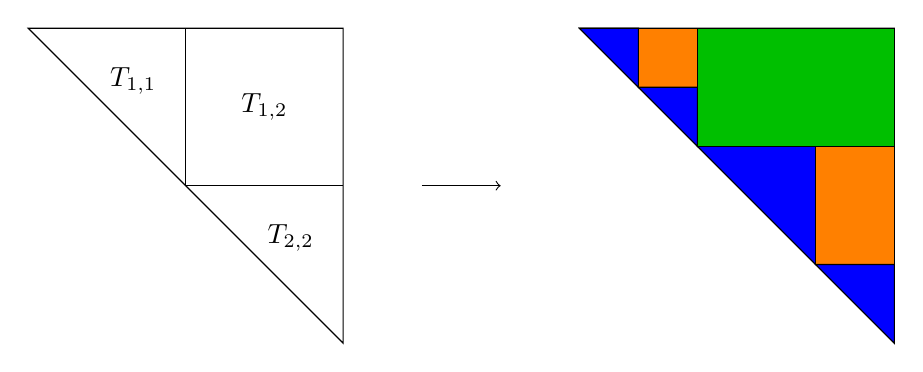
\begin{tikzpicture}
            \draw  (4,4) % Top right
                -- (4,0) % bottom right
                -- (0,4) % top left
                -- cycle;
            \draw  (2,4)
                -- (2,2)
                -- (4,2);
            \node at (1.333,3.333) {$T_{1,1}$};
            \node at (3,3) {$T_{1,2}$};
            \node at (3.333,1.333) {$T_{2,2}$};
            \draw[->] (5,2) -- (6,2);
            \draw (7, 4) -- (11,4) -- (11, 0) -- cycle;
            \draw[fill=blue] (7, 4) -- (7.75, 4) -- (7.75, 3.25) -- cycle;
            \draw[fill=orange]  (7.75,4) -- (8.5,4) -- (8.5,3.25) -- (7.75,3.25) -- cycle;
            \draw[fill=blue] (7.75, 3.25) -- (8.5, 3.25) -- (8.5, 2.5) -- cycle;
            %\draw[fill=orange]   -- (10,4) -- (10,2.5) --  -- cycle;
            \draw[fill=blue] (8.5,2.5) -- (10, 2.5) -- (10, 1) -- cycle;
            \draw[fill=orange] (10,2.5) -- (11,2.5) -- (11,1) -- (10,1) -- cycle;
            \draw[fill=blue] (10,1) -- (11,1) -- (11,0) -- cycle;
            \draw[fill=green!75!black] (8.5,4) -- (11,4) -- (11,2.5) -- (8.5,2.5) -- cycle;
        \end{tikzpicture}
    \end{center}
        \caption{Visual representation of the $2^\text{nd}$ layer in recursively computing $T$. The blue triangles
        work together to compute the orange portions. Then the triangles made by combining the blue and orange
        pieces finally compute the green piece}\label{fig:recCall}
    \end{figure}
    \begin{figure}
        \begin{center}
        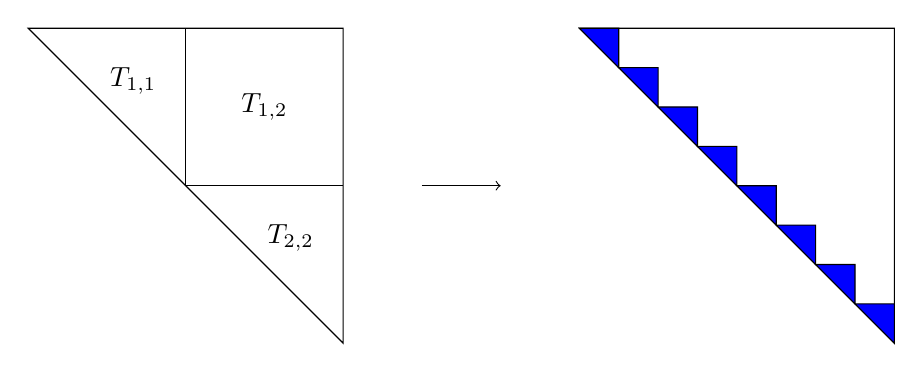
\begin{tikzpicture}
            \draw  (4,4) % Top right
                -- (4,0) % bottom right
                -- (0,4) % top left
                -- cycle;
            \draw  (2,4)
                -- (2,2)
                -- (4,2);
            \node at (1.333,3.333) {$T_{1,1}$};
            \node at (3,3) {$T_{1,2}$};
            \node at (3.333,1.333) {$T_{2,2}$};
            \draw[->] (5,2) -- (6,2);
            \draw (7, 4) -- (11,4) -- (11, 0) -- cycle;
            \draw[fill=blue] (7,4) -- (7.5,4) -- (7.5,3.5) -- cycle;
            \draw[fill=blue] (7.5,3.5) -- (8.0, 3.5) -- (8.0, 3.0) -- cycle;
            \draw[fill=blue] (8.0,3.0) -- (8.5, 3.0) -- (8.5, 2.5) -- cycle;
            \draw[fill=blue] (8.5,2.5) -- (9, 2.5) -- (9, 2) -- cycle;
            \draw[fill=blue] (9,2) -- (9.5, 2) -- (9.5, 1.5) -- cycle;
            \draw[fill=blue] (9.5,1.5) -- (10, 1.5) -- (10, 1) -- cycle;
            \draw[fill=blue] (10,1) -- (10.5, 1) -- (10.5, .5) -- cycle;
            \draw[fill=blue] (10.5, .5) -- (11, .5) -- (11, 0) -- cycle;
        \end{tikzpicture}
        \end{center}
        \caption{Visual representation of the terminating case in recursively computing $T$. Each of these blue
        triangles are set using our $\tau$ vector}\label{fig:termCase}
    \end{figure}
    \subsection{Matrix Operation LARFT}
    \begin{theorem}\label{thm:Puglisi}
        Theorem 2 in \cite{Joff}:

        Let $U\in\R^{m\times k}$ have linearly independent columns. Then, there exists
        a unique nonsingular upper triangular matrix $S\in\R^{k\times k}$ such that
        $I-USU^\top$ is an orthogonal matrix. This matrix $S$ satisfies $S=T^{-1}$ with
        $T+T^\top = U^\top U$, where $T\in\R^{k\times k}$ is itself a unique nonsingular upper 
        triangular matrix.
    \end{theorem}
    With this theorem coupled with work done in \cite{Puglisi}, we have an algorithm to compute the $T$ that 
    we need. This algorithm is heavily inspired by \cite{Joff} and is given by algorithm \ref{alg:UTDLARFT}

    \begin{algorithm}
        \caption{DLARFT implementation based on \cite{Joff} and \cite{Puglisi}}\label{alg:UTDLARFT}
        \begin{algorithmic}[1]
            \REQUIRE $V\in\R^{m\times n}, T\in\R^{n\times n}, \tau\in\R^n$\hfill\COMMENT{$m\geq n\geq 1$}
            \STATE $T = \text{upperTriangularPart}\left(V^\top V\right)$
            \FOR{ $i=1,\cdots n$ }
                \STATE $T(i,i) = \frac{T(i,i)}{2}$
            \ENDFOR
            \STATE 
        \end{algorithmic}
    \end{algorithm}
    \subsection{Numerical Experiments}
    We ran numerical experiments on the \href{https://ccm-docs.readthedocs.io/en/latest/alderaan/#hardware}{cluster}
    here at CUDenver. We can see the performance in figure \ref{fig:DLARFT}. The key takeaway is that our new
    scheme is roughly 3 times more performant than existing algorithms inside LAPACK as well as AOCL.
    \begin{figure}
        \centering
        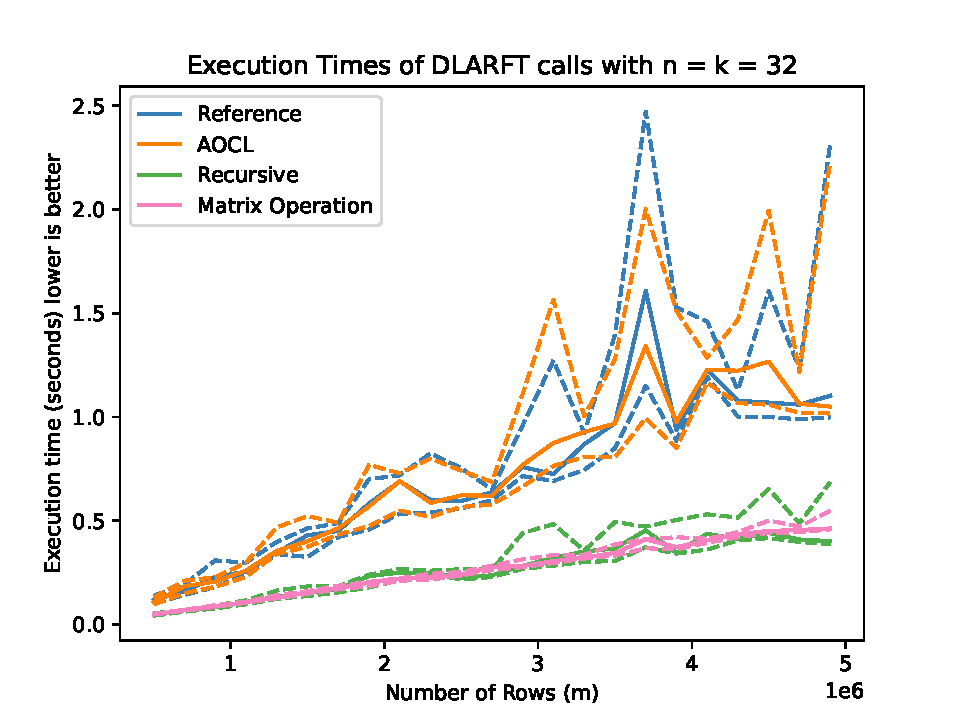
\includegraphics[width=.45\textwidth]{figures/timeDLARFT.pdf}
        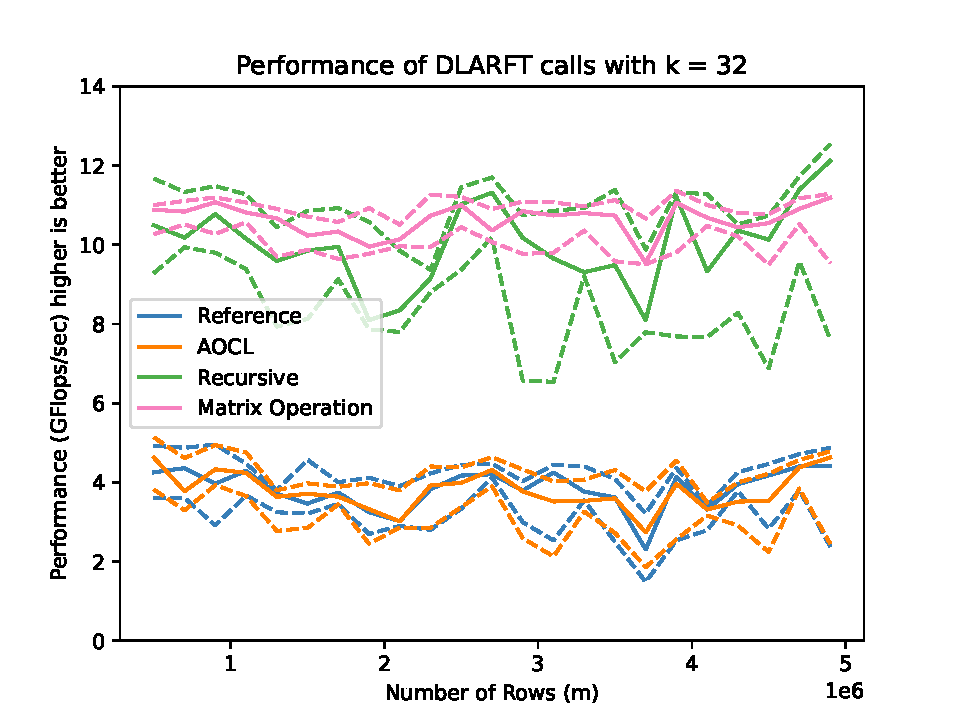
\includegraphics[width=.45\textwidth]{figures/flopDLARFT.pdf}
        \caption{Comparison of varying DLARFT versions with fixed $n$.}\label{fig:DLARFT}
    \end{figure}
    \subsection{Computational Cost}
    By looking at our implementation along with reference LAPACK, we get the following operation counts that are
    used in the previous figures.
    \[
    \begin{aligned}
            \text{DLARFT: }&\,      \frac{6mk^2 - 6mk -4k^3 +6k^2 - 2k}{6}&\approx mk^2 - \frac{2k^3}{3}\\
            \text{DLARFT\_REC: }&\, \frac{6mk^2 - 6mk -2k^3 +3k^2 -  k}{6}&\approx mk^2 - \frac{k^3}{3}\\
            \text{DLARFT\_MAT: }&\, \frac{6mk^2 + 6mk +4k^3 -9k^2 + 5k}{6}&\approx mk^2 + \frac{2k^3}{3}
    \end{aligned}
    \]
    \section{DLARFB}
    In order to apply the block of reflectors to our already formed columns of $Q$, we use \verb|DLARFB|.
    However the existing algorithm is a general one, which we will present first then discuss 
    specialization to our algorithm.
    \subsection{Existing behavior}
        Given $V\in\R^{m\times k}$, $T\in\R^{k\times k}$, and $C\in\R^{m\times n}$, we 
        want to compute $C = HC$ where $H$ has the form
        $$
        H = I - VTV^\top
        $$
        $V$ is unit lower triangular, $T$ is upper triangular, and $C$ is any matrix of the proper shape. 

        We also break up $V$ and $C$ as follows
        \begin{align}
            V &= \begin{bmatrix} V_1 \\ V_2 \end{bmatrix} \label{eq:vMatVert} \\
            C &= \begin{bmatrix} C_1 \\ C_2 \end{bmatrix} \label{eq:cMatVert}
        \end{align}
        Where $V_1\in\R^{k\times k}$ is unit lower triangular, and $C_1\in\R^{n\times n}$.

        By substituting in this breaking down of $C$ and $V$ into our equation $C = HC$, we can write each of the
        compenents as follows
        \begin{align*}
            C_1 &= C_1 - V_1T\left(V_1^\top C_1 + V_2^\top C_2\right) \\
            C_2 &= C_2 - V_2T\left(V_1^\top C_1 + V_2^\top C_2\right).
        \end{align*}
        Looking at this characterization, we can see that if we can exploit some fact of $C$ then we 
        can potentially help out our main driver.

        The current implementation is given by algorithm \ref{alg:refDLARFB}
        \begin{algorithm}
            \caption{Reference DLARFB}\label{alg:refDLARFB}
            \begin{algorithmic}[1]
                \REQUIRE $V\in\R^{m\times k}, T\in\R^{k\times k}, C\in\R^{m\times n}$
                \STATE $W = $ new matrix in $\R^{k\times k}$
                \STATE $W = C_1^\top$
                \STATE $W = WV_1$
                \STATE $W = W + C_2^\top V_2$
                \STATE $W = WT^\top$
                \STATE $C_2 = C_2 - V_2W^\top$
                \STATE $W = WV_1^\top$
                \STATE $C_1 = C_1 - W^\top$
            \end{algorithmic}
        \end{algorithm}
        
        However, for us, we get that $C_1$ is identically $0$, so lets try to exploit it, which we do in 
        algorithm \ref{alg:DLARFB0C2}
    \subsection{New Behavior}
    Since we get from algorithm \ref{alg:dorgqr} that $C_1 = 0$, it is of the same size as $W$ from 
    algorithm \ref{alg:refDLARFB}, and we will be overwriting it anyway, we can actually use this 
    region as a workspace, which gives us algorithm \ref{alg:DLARFB0C2}.
    \begin{algorithm}
        \caption{DLARFB\_0C2}\label{alg:DLARFB0C2}
        \begin{algorithmic}[1]
            \REQUIRE $V\in\R^{m\times k}, T\in\R^{k\times k}, C\in\R^{m\times n}$
            \STATE $C_1 = V_2^\top C_2$
            \STATE $C_1 = TC_1$
            \STATE $C_2 = C_2 - V_2C_1$
            \STATE $C_1 =     - V_1C_1$
        \end{algorithmic}
    \end{algorithm}
    \subsection{Flop Comparison}
    \section{Main Driver Algorithm}
    \subsection{Saving Flops on first iteration}
    \section{DORG2R}
    \subsection{What it is supposed to do}
    \subsection{Existing Behavior}
    \subsection{``Blocked'' equivalent}
    \section{DORGKR}
    \subsection{Algorithm Overview}
    \subsection{Numerical Experiments}
    \subsection{Computational Cost}
    \section{Putting it all together}
    \section{Source Code}
    The code for this software can be found in the repository \href{https://github.com/jprhyne/Fall23}{Fall23}
    \section{References}
    \bibliographystyle{plain}
    \bibliography{report}

\end{document}
